\documentclass[10pt,twocolumn,letterpaper]{article}

\usepackage{cvpr}
\usepackage{times}
\usepackage{epsfig}
\usepackage{graphicx}
\usepackage{amsmath}
\usepackage{amssymb}
\usepackage{booktabs}
\usepackage{tikz}
\usetikzlibrary{arrows.meta, positioning}

\usepackage[breaklinks=true,bookmarks=false]{hyperref}

\cvprfinalcopy

\def\cvprPaperID{0000}
\def\httilde{\mbox{\tt\raisebox{-.5ex}{\symbol{126}}}}

\graphicspath{{figures/}}

\newcommand{\good}[1]{#1}

\begin{document}

%%%%%%%%% TITLE
\title{Breaking the Rollout Wall: A Discrete-Token World Model for Atari Breakout}

\author{Mingyang Li\\
ICME\\
{\tt\small mili1@stanford.edu}
}

\maketitle

%%%%%%%%% ABSTRACT
\begin{abstract}
We study \emph{action-conditioned world models} that learn to simulate Atari
Breakout: given a few starting frames and a sequence of actions, the model
should generate a coherent, game-like continuation. We first build a
deterministic next-frame predictor---a convolutional U-Net with
feature-wise linear modulation (FiLM) for action conditioning and a bounded
residual decoder---and show that, while it learns clean one-step predictions,
it cannot produce stable autoregressive rollouts. We characterize this failure
precisely: under closed-loop generation the model's error compounds, and the
\emph{type} of collapse (brightness blow-up vs.\ motion freeze) is controlled
entirely by a single regularization weight, with no stable setting in between.
This is the classic exposure-bias wall of pixel-regression models. Motivated by
this analysis, we switch to a two-stage discrete-token model in the style of
recent transformer world models: a VQ-VAE tokenizer encodes each
$128\times128$ frame into a $16\times16$ grid of discrete codes, and a GPT-style
causal transformer models the next-frame tokens conditioned on past tokens and
actions, trained with cross-entropy and generated by temperature sampling. The
token model produces coherent rollouts over the full clip with no blow-up or
freeze, and---because generation is stochastic---different samples from the same
prime yield different plausible futures. We further diagnose a ball-respawn
limitation as a \emph{data-coverage} problem rather than a modeling failure and
fix it at the data-collection level. Our results align with our hypothesis:
L1 pixel regression hits a fundamental rollout wall, while discrete tokenization
plus autoregressive sampling breaks it.
\end{abstract}

%%%%%%%%% BODY
\section{Introduction}

A \emph{world model} learns the dynamics of an environment: given the recent
history of observations and an action, it predicts the next observation. If the
predictions are accurate and stable, the model can be unrolled to ``imagine''
entire trajectories, which is useful for planning, model-based reinforcement
learning, and as a learned simulator~\cite{ha2018worldmodels,hafner2020dreamer}.
We study this problem on Atari Breakout, where the dynamics---a ball bouncing off
a paddle and walls, breaking bricks---are simple to describe but surprisingly
hard to generate frame-by-frame, because the ball is only one or two pixels wide
at the resolutions practical for training.

Our goal is concrete: prime the model with a few real frames plus a sequence of
actions, and roll out a clip that ``looks like someone is playing the game.''
The central difficulty is not one-step prediction but \emph{autoregressive
rollout}: when the model consumes its own predictions, small errors compound.

We make two contributions. First, we build a strong deterministic baseline---a
FiLM-conditioned U-Net with a bounded residual decoder---and show through
controlled experiments that it learns clean one-step predictions yet cannot roll
out stably. We characterize the failure as a trade-off between two collapse
modes governed by a single brightness-regularization weight, with no stable
operating point, and argue this is the exposure-bias wall inherent to pixel
regression. Second, motivated by this analysis, we implement a discrete-token
world model (VQ-VAE tokenizer + causal transformer) and show it produces
coherent, \emph{stochastic}, action-conditioned rollouts that the deterministic
model cannot. We also present an honest failure analysis (ball respawn) and a
data-level fix. The result is both a working model and a clear story about
\emph{why} the simpler approach fails.

\section{Related Work}

\textbf{Latent world models.} Ha and Schmidhuber~\cite{ha2018worldmodels}
introduced the encoder--dynamics--decoder template that we follow. The
PlaNet/Dreamer line~\cite{hafner2019planet,hafner2020dreamer,hafner2021dreamerv2,
hafner2023dreamerv3} uses a recurrent state-space model with a \emph{stochastic}
latent and a KL objective; DreamerV2~\cite{hafner2021dreamerv2} notably switched
to \emph{discrete} (categorical) latents for Atari, supporting our finding that
discreteness helps. SimPLe~\cite{kaiser2020simple} learns a pixel-space
video-prediction model for Atari and is closest to our deterministic baseline.

\textbf{Token / generative world models.} IRIS~\cite{micheli2023iris} tokenizes
frames with a VQ-VAE~\cite{oord2017vqvae} and models dynamics with a transformer
over tokens; our token model is a minimal version of this design. Image
GPT~\cite{chen2020igpt} established autoregressive transformers over image
tokens. DIAMOND~\cite{alonso2024diamond}, GameNGen~\cite{valevski2024gamengen},
and Genie~\cite{bruce2024genie} use diffusion or large transformers for
high-fidelity playable world models; these are far beyond our compute budget but
share the core idea that strong generative decoders avoid the blur of pixel
regression.

\textbf{Components.} Our deterministic model uses a U-Net~\cite{ronneberger2015unet}
for spatial detail and FiLM~\cite{perez2018film} for action conditioning. The
transformer follows the standard causal architecture~\cite{vaswani2017attention}.
Compared with these works, we claim no architectural novelty: our token model is
a deliberately minimal reimplementation of the IRIS recipe (VQ-VAE\,+\,causal
transformer), and the broad conclusion that discrete latents help on Atari was
already established by IRIS~\cite{micheli2023iris} and
DreamerV2~\cite{hafner2021dreamerv2}. What we contribute, as a course project, is
a \emph{controlled, single-pipeline comparison} that those papers do not report:
holding the data, environment, and evaluation fixed, we show \emph{why} the
deterministic baseline fails by characterizing its failure as a
regularization-controlled blow-up$\leftrightarrow$freeze trade-off
(\S\ref{sec:det}), and we measure the token model on the \emph{same} rollout axes
to confirm it stays on ground truth where the baseline cannot. We treat this as a
pedagogical, reproducible demonstration rather than a new method.

\section{Data}

We collect trajectories from Atari Breakout via the Arcade Learning
Environment~\cite{bellemare2013ale} (\texttt{ALE/Breakout-v5}). Each frame is
converted to grayscale and resized to $128\times128$ with nearest-neighbor
sampling (we initially used $64\times64$ and increased resolution to sharpen the
1--2 pixel ball). An observation \emph{state} is a stack of the last four frames,
which provides velocity information. We record the discrete action at each step
(4 actions, one-hot encoded).

Trajectories are gathered with a random policy and a frame skip of 2 for visual
diversity. Each episode begins with a \texttt{FIRE} action to launch the ball,
and we discard near-static clips (max inter-frame difference below a threshold).
Our main dataset is 2{,}000 sequences of length 50 ($100{,}000$ frames). Because
the world model trains per-frame for the tokenizer and on windows of frames for
the dynamics model, this provides ample supervision.

\textbf{Targeted respawn coverage.} Breakout's life-loss mechanic requires the
agent to press \texttt{FIRE} to launch a new ball after one is lost; with a pure
random policy and short clips, a full
``ball lost $\rightarrow$ \texttt{FIRE} $\rightarrow$ respawn'' cycle rarely
appears, so a world model trained on such data has no chance of learning it. We
explicitly address this at the collection level: we monitor the environment's
life counter and, whenever a life is lost, force the next action to be
\texttt{FIRE}, combined with longer (length-50) clips. With this policy, 9 of 10
collected sequences contain a complete respawn cycle, giving the world model the
supervision needed to reproduce the mechanic faithfully.

\section{Methods}

\subsection{Overview}
We compare two models that share the framing ``predict the next frame from a
4-frame stack and an action,'' but differ in representation and objective
(Figure~\ref{fig:arch}).

\begin{figure}[t]
\centering
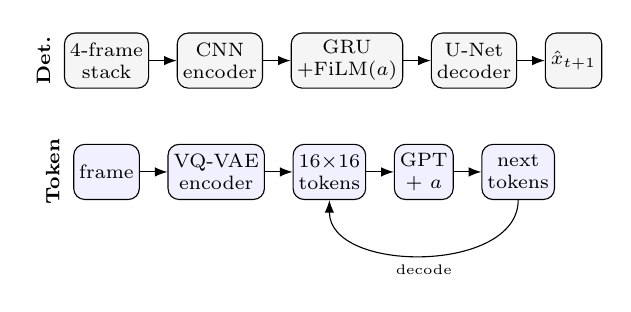
\begin{tikzpicture}[
  box/.style={draw, rounded corners, align=center, font=\scriptsize,
              minimum height=0.7cm, inner sep=2pt},
  ar/.style={-{Latex[length=1.6mm]}}, font=\scriptsize, node distance=0.35cm]
% deterministic row
\node[box, fill=black!4] (a1) {4-frame\\stack};
\node[box, right=of a1, fill=black!4] (a2) {CNN\\encoder};
\node[box, right=of a2, fill=black!4] (a3) {GRU\\+FiLM($a$)};
\node[box, right=of a3, fill=black!4] (a4) {U-Net\\decoder};
\node[box, right=of a4, fill=black!4] (a5) {$\hat{x}_{t+1}$};
\draw[ar](a1)--(a2); \draw[ar](a2)--(a3); \draw[ar](a3)--(a4); \draw[ar](a4)--(a5);
\node[left=0.05cm of a1, font=\scriptsize\bfseries, rotate=90, anchor=south]{Det.};
% token row
\node[box, below=0.7cm of a1, fill=blue!6] (b1) {frame};
\node[box, right=of b1, fill=blue!6] (b2) {VQ-VAE\\encoder};
\node[box, right=of b2, fill=blue!6] (b3) {$16{\times}16$\\tokens};
\node[box, right=of b3, fill=blue!6] (b4) {GPT\\+ $a$};
\node[box, right=of b4, fill=blue!6] (b5) {next\\tokens};
\draw[ar](b1)--(b2); \draw[ar](b2)--(b3); \draw[ar](b3)--(b4); \draw[ar](b4)--(b5);
\draw[ar](b5) to[out=-90,in=-90] node[below,font=\tiny]{decode} (b3);
\node[left=0.05cm of b1, font=\scriptsize\bfseries, rotate=90, anchor=south]{Token};
\end{tikzpicture}
\caption{Two approaches. \textbf{Top:} deterministic FiLM U-Net regresses the
next frame. \textbf{Bottom:} a VQ-VAE tokenizes frames and a causal transformer
predicts next-frame tokens, decoded back to pixels.}
\label{fig:arch}
\end{figure}

\subsection{Deterministic FiLM U-Net}
A convolutional encoder maps the 4-frame stack to a latent $z_t$ and a set of
spatial skip features. A GRU advances the latent conditioned on the action,
$z_{t+1}=\mathrm{GRU}([z_t, e(a_t)])$, and a U-Net decoder with skip connections
produces the output. We found two design choices essential. (i)~\textbf{Skip
connections}~\cite{ronneberger2015unet}: a flat 256-d latent cannot encode a
1-pixel ball location, so a pure bottleneck produces a blurry, fading ball; skips
route pixel detail to the decoder. (ii)~\textbf{FiLM action conditioning}~\cite{perez2018film}:
concatenating a 4-d action to a 256-d latent makes the action negligible and the
model ignores it; instead we modulate every decoder feature map with per-channel
scale and bias predicted from the action, $h \!\leftarrow\! (1+\gamma(a))\,h +
\beta(a)$, initialized to identity. The decoder predicts a bounded residual,
$\hat{x}_{t+1}=\mathrm{clip}(x_t + s\cdot\tanh(\delta),0,1)$, which keeps
predictions anchored to the previous frame.

The model is trained with a motion-aware loss that up-weights changed and bright
pixels, plus a delta term, a false-motion penalty, and a brightness-conservation
term that penalizes per-frame mean-intensity drift:
\begin{align}
\mathcal{L} =\;& \mathbb{E}\big[w \cdot \mathrm{SmoothL1}(\hat{x},x^\star)\big]
  + \lambda_1\,\mathcal{L}_{\Delta} \nonumber\\
  &+ \lambda_2\,\mathcal{L}_{\text{false-mot}}
  + \lambda_3\,\mathcal{L}_{\text{bright}} .
\end{align}

\subsection{Discrete-token world model}
\textbf{Tokenizer.} A VQ-VAE~\cite{oord2017vqvae} encodes each $128\times128$
grayscale frame to an $8\times$-downsampled $16\times16$ grid; each cell is
quantized to its nearest entry in a codebook of $K{=}512$ vectors, giving
$256$ discrete tokens per frame. We use an exponential-moving-average codebook
for stability and an object-weighted reconstruction loss so the small bright ball
survives quantization. The tokenizer is fully convolutional, so changing input
resolution requires no architectural change.

\textbf{Dynamics.} A GPT-style causal transformer~\cite{vaswani2017attention,
chen2020igpt} models the flattened, action-interleaved token sequence
$[f_0,a_0,f_1,a_1,\dots]$, where each $f_t$ is the $256$ tokens of frame $t$ and
$a_t$ is an action token placed immediately before frame $t{+}1$. We train with
next-token cross-entropy, supervising only frame-token positions (actions are
control inputs). At generation we sample frame tokens with temperature and
top-$k$, decode them with the frozen tokenizer, and slide a context window so
rollouts can exceed the training context length. A key-value cache makes
generation roughly an order of magnitude faster.

\textbf{Why tokens.} Cross-entropy over discrete codes does not average distinct
futures into a blur the way L1 regression does, and discrete codes cannot
gradually decay in intensity---the two mechanisms behind the deterministic
model's rollout failure. Sampling additionally yields stochastic futures.

\section{Experiments}

\subsection{Setup and metrics}
All models are trained with AdamW. The deterministic model ($\sim$10.4M params)
trains on a single GPU; the tokenizer ($\sim$6.2M params) and transformer
($\sim$26.8M params) train on an A100. We evaluate: (1) one-step teacher-forced
quality; (2) \emph{rollout coherence}---whether motion persists and the image
stays valid under closed-loop generation; (3) brightness stability (max pixel
over the rollout); (4) action sensitivity, $\|\hat{x}(a_i)-\hat{x}(a_j)\|$; and
(5) stochasticity, whether samples from the same prime diverge. Baselines are
copy-last-frame and ablations of the deterministic model. Model hyperparameters
are listed in Table~\ref{tab:hp}.

\begin{table}[t]
\centering\footnotesize
\renewcommand{\arraystretch}{1.1}
\begin{tabular}{ll}
\multicolumn{2}{c}{\textbf{(a) Deterministic FiLM U-Net}}\\
\toprule
input stack & 4 frames, $64\!\times\!64$ \\
latent / hidden  dim & 256 / 512 \\
action embed dim & 128 \\
decoder & U-Net, residual head \\
residual scale $s$ & 0.2 \\
loss weights $\lambda_1,\lambda_2,\lambda_3$ & 100, 50, 8 \\
optimizer / lr & AdamW, $10^{-4}$ \\
params & $\sim$10.4M \\
\midrule[\heavyrulewidth]
\multicolumn{2}{c}{\textbf{(b) VQ-VAE tokenizer}}\\
\toprule
input frame & $128\!\times\!128$ grayscale \\
token grid & $16\!\times\!16$ ($P{=}256$) \\
codebook size $K$ & 512 \\
embedding dim $D$ & 256 \\
commitment cost & 0.25 \\
EMA decay & 0.99 \\
object weight (recon) & 30 \\
optimizer / lr & AdamW, $3\!\cdot\!10^{-4}$ \\
params & $\sim$6.2M \\
\midrule[\heavyrulewidth]
\multicolumn{2}{c}{\textbf{(c) GPT dynamics}}\\
\toprule
vocabulary & 512 frame + 4 action \\
context frames & 8 \\
$d_{\text{model}}$ / layers / heads & 512 / 8 / 8 \\
dropout & 0.1 \\
batch size & 16 \\
optimizer / lr & AdamW, $3\!\cdot\!10^{-4}$ \\
weight decay & 0.01 \\
sampling & temperature 1.0, top-$k$ 50 \\
params & $\sim$26.8M \\
\bottomrule
\end{tabular}
\caption{Hyperparameters for the three models.}
\label{tab:hp}
\end{table}

\subsection{The deterministic model hits a wall}
\label{sec:det}
The deterministic model learns clean one-step teacher-forced predictions, and
FiLM is necessary for it to use the action: action sensitivity rises from exactly
$0.000$ (concatenation) to $\sim$0.20 (FiLM). However, free rollout fails, and
the failure \emph{mode} is governed by the brightness-regularization weight
(Figure~\ref{fig:det}). With weak regularization the prediction's maximum pixel
value climbs from $0.58$ to $1.0$ within $\sim$6 frames and the screen whites out
(\emph{blow-up}). With strong regularization the per-frame motion collapses from
$\sim$12 to $\sim$1 and the frame freezes (\emph{freeze}). Crucially, no
intermediate setting is stable---tuning trades one failure for the other. We also
observed, earlier in development, copy-last-frame collapse and mode collapse to a
mean ``brick-wall'' frame, all consistent with the same underlying cause: L1
regression cannot represent multi-modal futures and has no mechanism to halt
intensity drift in closed loop.

\begin{figure}[t]
\centering

\includegraphics[width=0.8\linewidth]{fs_blowup}\\[2pt]
{\footnotesize (a) Blow-up: max pixel $0.58\!\to\!1.0$, screen whites out}\\[4pt]

\includegraphics[width=0.99\linewidth]{fs_freeze}\\[2pt]
{\footnotesize (b) Freeze: motion $\sim$12$\to$1, ball dies}
\caption{Deterministic rollout failure (frames left$\to$right). The collapse mode
is set by the brightness-regularization weight; there is no stable setting.}
\label{fig:det}
\end{figure}

\begin{figure}[t]
\centering
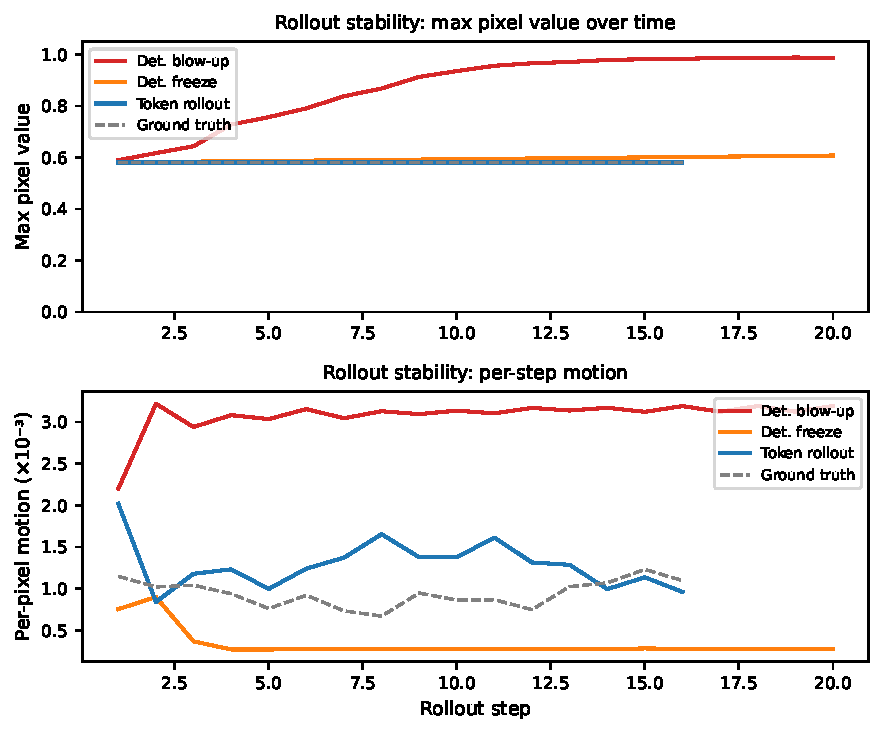
\includegraphics[width=0.8\linewidth]{coherence_plot_vertical}
\caption{Quantitative rollout comparison, averaged over 30 held-out sequences.
\textbf{Top (max pixel):} under weak brightness-regularization the deterministic
prediction saturates toward $1.0$ (red, blow-up); under strong regularization it
stays flat (orange, freeze). \textbf{Bottom (per-step motion):} the blow-up
regime keeps high but meaningless motion ($\sim$3$\times10^{-3}$), while the
freeze regime collapses to near-zero ($\sim$0.3$\times10^{-3}$). In both panels
the \emph{token rollout} (blue) tracks the ground-truth band (grey dashed) for
the full clip---stable brightness around $0.58$ and motion in the healthy GT
range---whereas both deterministic regimes leave the GT band within
$\sim$6 steps. The token model is the only one that stays on GT on both axes.}
\label{fig:coh}
\end{figure}

A quantitative view of the same phenomenon is in Figure~\ref{fig:coh}. Both
deterministic regimes diverge from the ground-truth bands within $\sim$6 rollout
steps, on either the brightness or the motion axis. Crucially the deviations are
\emph{monotonic}---blow-up keeps rising and freeze stays dead---demonstrating that
the failure compounds rather than self-corrects.

\subsection{The token model produces coherent rollouts}
The VQ-VAE reaches a reconstruction loss of $0.0034$ at $128\times128$ with the
ball and paddle clearly reconstructed (Figure~\ref{fig:recon}). The transformer
trains from a cross-entropy of $0.30$ down to $0.0084$. As shown in
Figure~\ref{fig:tok}, rollouts primed on four real frames stay \emph{coherent
over the full clip}: the ball moves and bounces, the paddle tracks, and bricks
persist---no blow-up and no freeze. Crucially, we evaluate the token model on the
\emph{same} axes used to diagnose the deterministic failure
(Figure~\ref{fig:coh}, blue): averaged over 30 held-out sequences, its max pixel
stays flat at $\approx$0.58 (matching ground truth, vs.\ the blow-up regime's
drift to $1.0$) and its per-step motion stays within the ground-truth band
($\approx$1$\times10^{-3}$, vs.\ the freeze regime's collapse to
$\approx$0.3$\times10^{-3}$). Unlike both deterministic regimes, which leave the
GT band within $\sim$6 steps, the token rollout never diverges over the full
clip---turning the qualitative ``coherent'' claim into a measured one.

\textbf{Codebook utilization.} Encoding 200 sequences ($1.02$M token slots), we
find only $7$ of the $512$ codes are ever used, with an empirical perplexity of
$4.9$; the top two codes cover $65\%$ of all tokens and the top five cover $95\%$
(Figure~\ref{fig:codebook}). This is \emph{expected} for low-entropy Breakout
frames rather than a sign of harmful codebook collapse: most $8\!\times\!8$
patches are pure background or uniform brick texture, so few distinct codes are
\emph{needed}. Two pieces of evidence rule out a degenerate ``lookup-table''
explanation. First, reconstruction is faithful---the one- to two-pixel ball,
paddle, and bricks all survive quantization (Figure~\ref{fig:recon})---which a
handful of indistinct codes could not achieve. Second, the representation is not
$5$ codes but a $16\!\times\!16$ \emph{spatial grid} of $256$ cells each drawn
from this small alphabet, so ball position is encoded by \emph{where} the
foreground code appears, not by code identity alone. Third, the active codes are
genuinely distinct: their embedding vectors have a mean pairwise distance of
$4.2$ (minimum $1.8$), so they are well-separated rather than collapsed onto a
single point. The small alphabet thus reflects the data's low visual entropy, not
a degenerate encoder.

\begin{figure}[t]
\centering
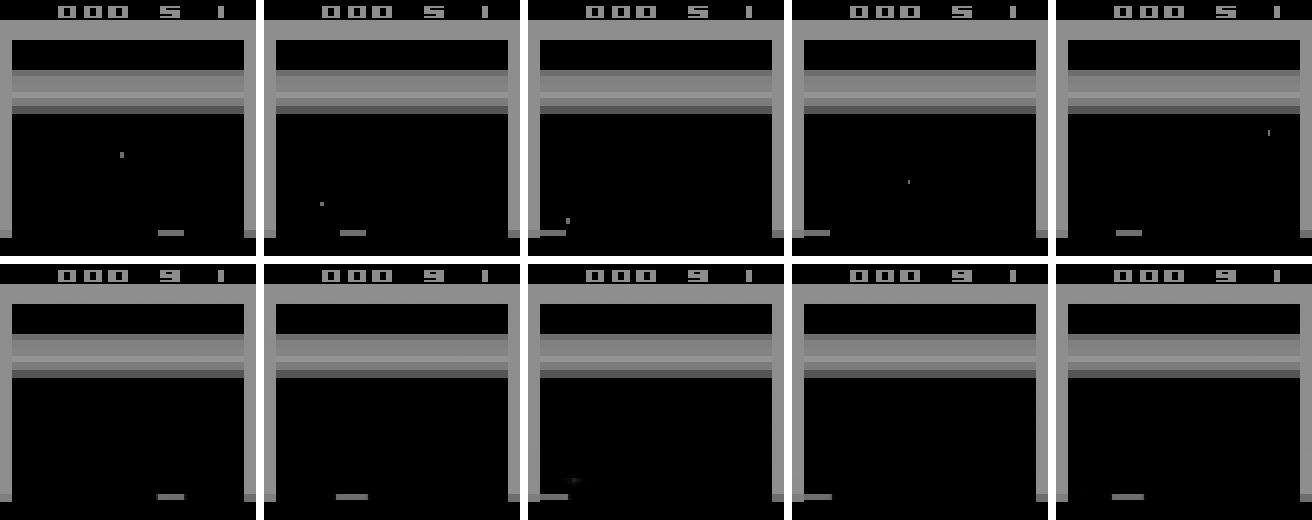
\includegraphics[width=0.99\linewidth]{fs_recon}
\caption{VQ-VAE reconstruction quality at $128\!\times\!128$. \textbf{Top row:}
ground-truth frames; \textbf{bottom row:} reconstructions through the
$16\!\times\!16$ token grid. Bricks, paddle, and the small bright ball all
survive quantization, confirming the discrete representation preserves the
information the dynamics model needs.}
\label{fig:recon}
\end{figure}

\begin{figure}[t]
\centering
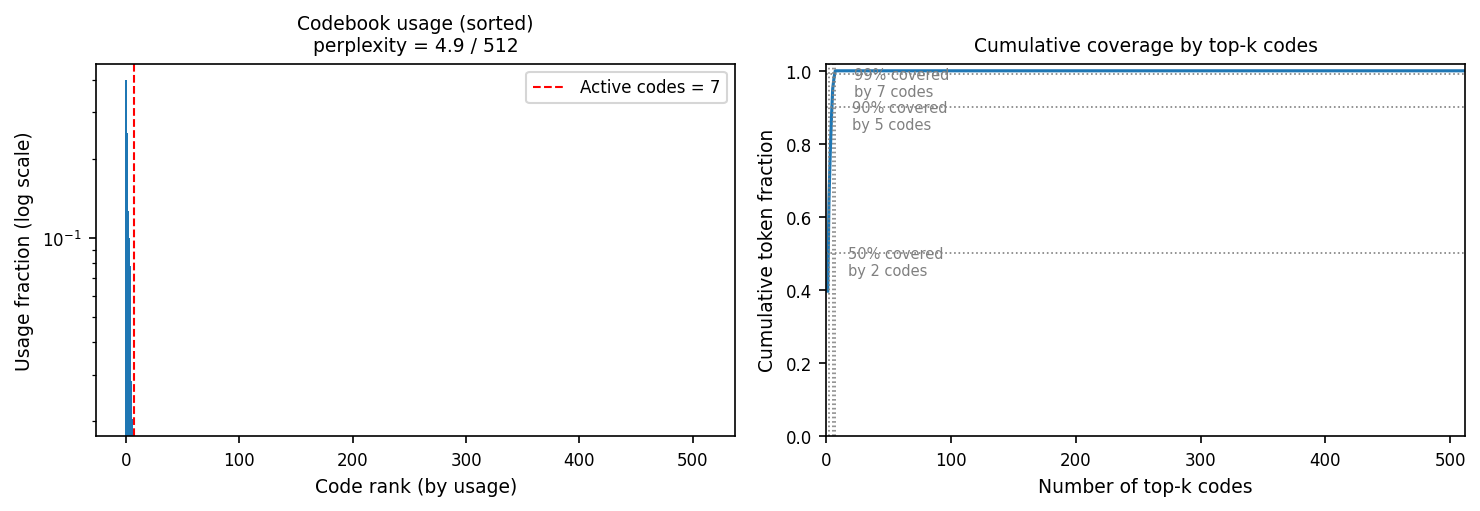
\includegraphics[width=0.99\linewidth]{codebook_usage}
\caption{Codebook utilization over $1.02$M encoded token slots. \textbf{Left:}
usage fraction per code (sorted, log scale)---only $7$ of $512$ codes are active.
\textbf{Right:} cumulative coverage; the top two codes account for $65\%$ and the
top five for $95\%$ of all tokens. The low perplexity ($4.9$) reflects the
genuinely low visual entropy of Breakout frames, not codebook collapse:
reconstruction stays faithful (Figure~\ref{fig:recon}) and the $16\!\times\!16$
spatial grid encodes object position by location, not code identity.}
\label{fig:codebook}
\end{figure}

\begin{figure}[t]
\centering
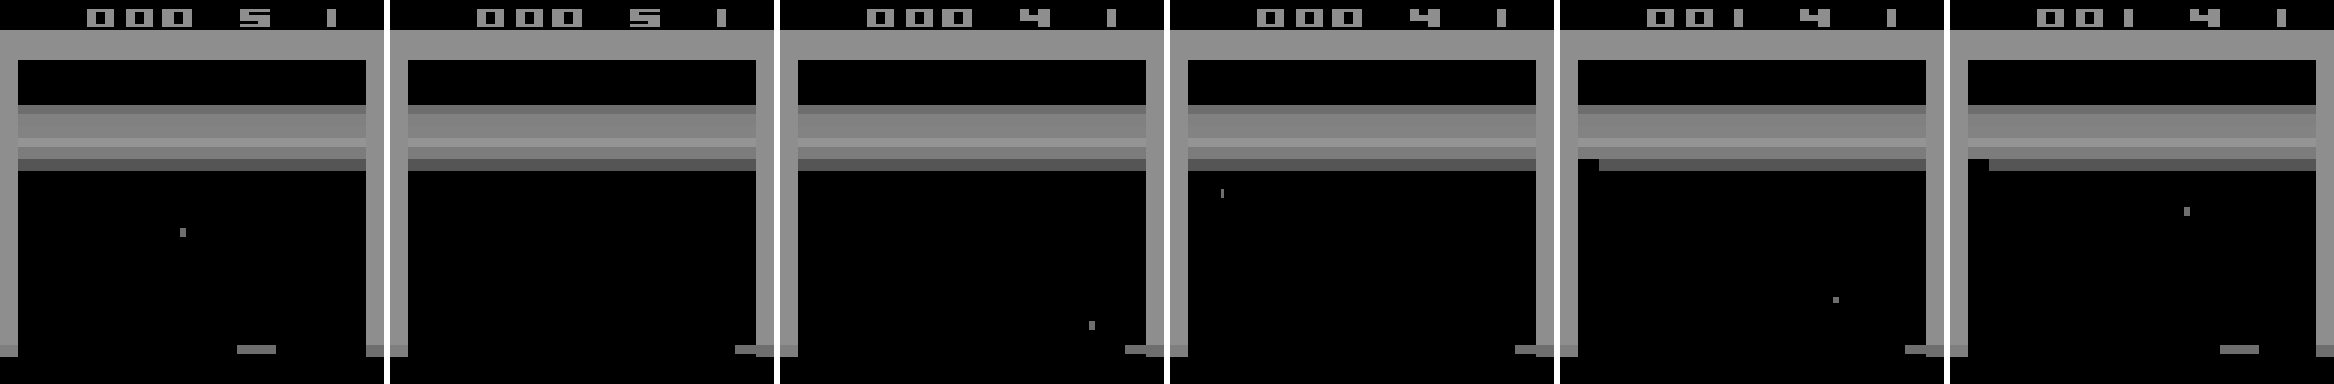
\includegraphics[width=0.99\linewidth]{fs_gt}\\[2pt]
{\footnotesize (a) Ground truth}\\[4pt]
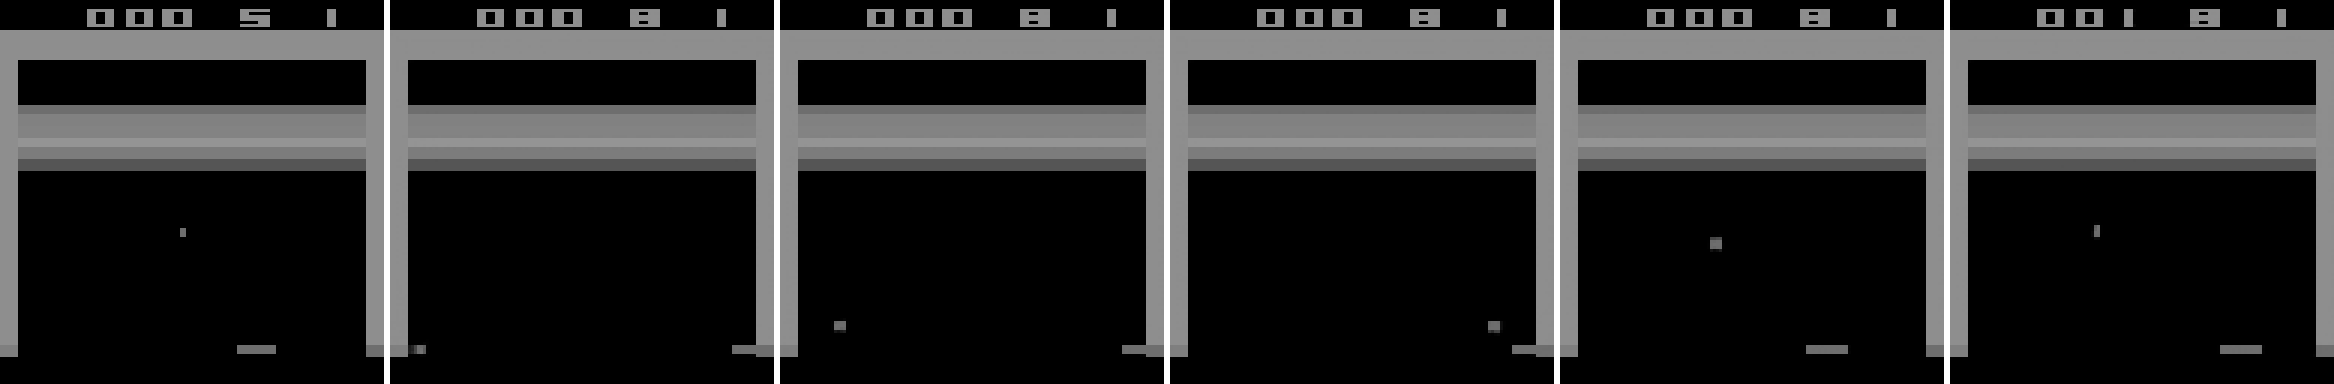
\includegraphics[width=0.99\linewidth]{fs_token}\\[2pt]
{\footnotesize (b) Token rollout (prime = 4 frames, then generated)}
\caption{The token world model produces a coherent rollout that tracks ground
truth, with stable brightness and persistent motion.}
\label{fig:tok}
\end{figure}

\begin{table}[t]
\centering\footnotesize
\renewcommand{\arraystretch}{1.2}
\begin{tabular}{lccc}
\toprule
 & Copy-last & Det.\ U-Net & Token \\
\midrule
One-step (TF)               & static & clean & clean \\
Coherent rollout (frames)   & 0      & $\sim$6 & full clip ($\geq$16) \\
Max pixel @ step 16         & 0.58   & 1.00 (blow-up) & 0.58 \\
Motion @ step 16 ($\times10^{-3}$) & 0 & 0.3 (freeze) & 1.0 \\
GT-band tracking            & no     & no    & both axes \\
Stochastic futures          & no     & no    & yes \\
\bottomrule
\end{tabular}
\caption{Comparison across our evaluation axes; rollout numbers averaged over 30
held-out sequences (Figure~\ref{fig:coh}). Ground-truth references are max
pixel $\approx$0.58 and motion $\approx$1$\times10^{-3}$. The deterministic
column reports its two failure regimes (blow-up on brightness, freeze on motion);
the token model is the only one that stays in the GT band on \emph{both} axes
\emph{and} produces diverse futures.}
\label{tab:cmp}
\end{table}

\subsection{Stochasticity}
Because generation samples from the predicted token distribution, the same prime
yields different futures. Figure~\ref{fig:stoch} shows three rollouts from
identical priming frames with different random seeds; at matched timesteps the
ball follows different trajectories, indicating the model learned a
\emph{distribution} over futures rather than a single continuation. This is the
action-conditioned stochastic simulation we set out to build, and a capability
the deterministic model fundamentally lacks (Table~\ref{tab:cmp}).

\begin{figure}[t]
\centering
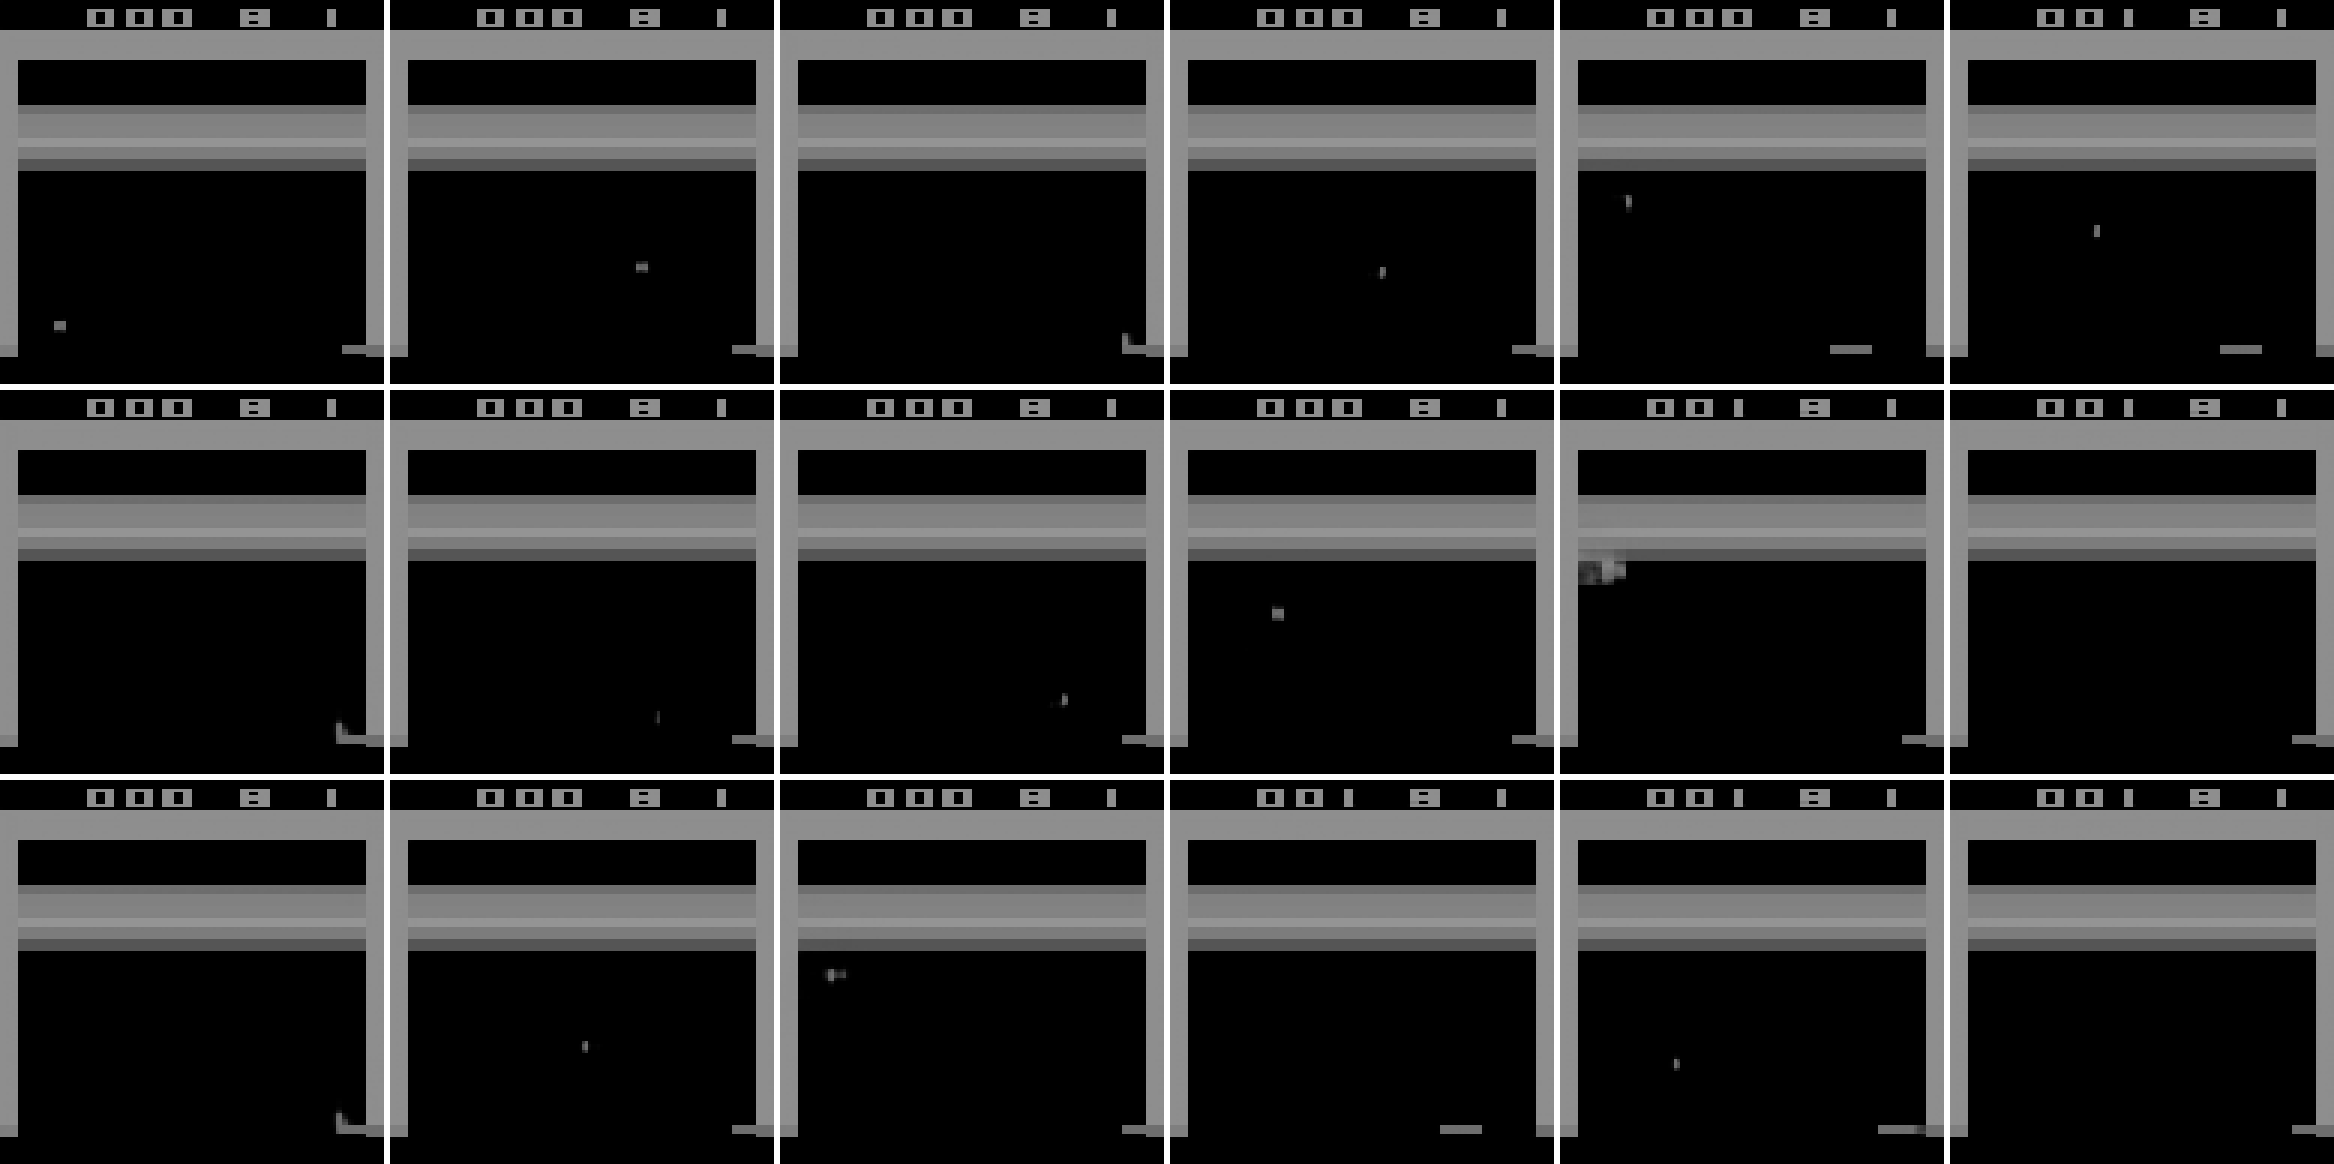
\includegraphics[width=0.99\linewidth]{fs_stochastic}
\caption{Three rollouts (rows) from the \emph{same} prime, different seeds.
Columns are matched timesteps; trajectories diverge, showing learned stochastic
dynamics.}
\label{fig:stoch}
\end{figure}

\subsection{Ablations}
Two ablations of the deterministic model isolate our design choices.
\emph{Removing skip connections} reverts the model to a flat bottleneck and
produces blurry, fading objects, confirming skips are needed for sub-pixel
spatial detail. \emph{Replacing FiLM with concatenation} drives action
sensitivity to exactly $0.000$---the model ignores the action---whereas FiLM
yields $\sim$0.20. For the token model, the brightness-conservation term and
residual-scale tuning that were critical for the deterministic model are
\emph{unnecessary}: discreteness removes the intensity-drift failure entirely.

\section{Conclusion}
We presented a controlled study of action-conditioned world modeling on Atari
Breakout. A deterministic FiLM U-Net learns clean one-step predictions but cannot
roll out stably: its failure is a regularization-controlled trade-off between
brightness blow-up and motion freeze, with no stable operating point---the
exposure-bias wall of pixel regression. A two-stage discrete-token model
(VQ-VAE + causal transformer) breaks this wall, producing coherent rollouts and,
through sampling, genuinely stochastic action-conditioned futures. We additionally
showed that a salient failure (ball respawn) is a data-coverage issue and fixed it
at the source. Future work includes quantifying the coherence horizon against
ground truth with per-frame error curves, temperature/top-$k$ ablations, color
(RGB) frames for visual realism, and extending to additional games. More broadly,
our results reinforce a lesson from recent world-model literature: the
representation and objective---discrete tokens with classification and
sampling---matter more for stable, diverse rollouts than tuning a pixel-regression
loss.

{\small
\bibliographystyle{ieee}
\bibliography{references}
}

\end{document}